\documentclass[conference]{IEEEtran}
\IEEEoverridecommandlockouts
\usepackage{cite}
\usepackage{amsmath,amssymb,bm}
\usepackage{booktabs}
\usepackage[table]{xcolor}
\usepackage{graphicx}
\usepackage{tikz}
\usetikzlibrary{positioning,arrows.meta,fit,backgrounds,calc,shapes.misc}
\usepackage{hyperref}
\hypersetup{colorlinks=true,linkcolor=black,citecolor=black,urlcolor=black}

% palette (same hues as the figures and charts)
\definecolor{cPrior}{HTML}{2A78D6}   % geometry prior
\definecolor{cInit}{HTML}{1BAF7A}    % initialisation
\definecolor{cModel}{HTML}{5B636E}   % 4D Gaussian model
\definecolor{cLoss}{HTML}{EB6834}    % objective
\definecolor{cEval}{HTML}{7A5BC7}    % evaluation
\definecolor{ink}{HTML}{12161B}

\tikzset{
  blk/.style={draw=#1, fill=#1!8, rounded corners=2pt, line width=0.6pt, align=center,
              font=\scriptsize, inner sep=2.5pt, minimum height=7mm, text=ink},
  io/.style={draw=ink!55, fill=white, rounded corners=2pt, line width=0.5pt, align=center,
             font=\scriptsize, inner sep=2.5pt, minimum height=7mm, text=ink},
  arr/.style={-{Stealth[length=2.2mm]}, line width=0.6pt, draw=ink!75},
  darr/.style={-{Stealth[length=2.2mm]}, line width=0.6pt, draw=ink!45, dashed},
  lane/.style={draw=#1!45, fill=#1!3, rounded corners=4pt, line width=0.4pt, inner sep=4pt},
  lanelbl/.style={font=\scriptsize\bfseries, text=#1, anchor=north west},
}

\begin{document}

\title{Getting the Surface Right: Scale-Corrected Monocular Geometry Priors for Endoscopic 4D Gaussian Splatting}
\author{\IEEEauthorblockN{Author Name(s)}\IEEEauthorblockA{Affiliation, City, Country \quad email@domain}}
\maketitle

\setcounter{section}{2}
\section{Methodology}
\label{sec:method}

Fig.~\ref{fig:pipeline} gives an overview. From a monocular endoscopic video with known camera poses, we (i)~correct the camera intrinsics, (ii)~predict a metric depth prior with MoGe-2~\cite{wang2025moge2}, (iii)~estimate its scale from the known poses and inter-frame matches (on P1; on the static P2\_5 clip from stereo), (iv)~initialise deformable 4D Gaussians from the scaled prior, and (v)~optimise them without the depth-related loss terms. The reconstruction architecture is that of Endo-4DGS~\cite{huang2024endo4dgs,wu2024_4dgs}; our changes concern the camera model, the depth prior, its scale and the training objective. Section~\ref{sec:evalproto} describes how we measure agreement with stereo-reference depth.

\begin{figure*}[t]
\centering
\resizebox{\textwidth}{!}{%
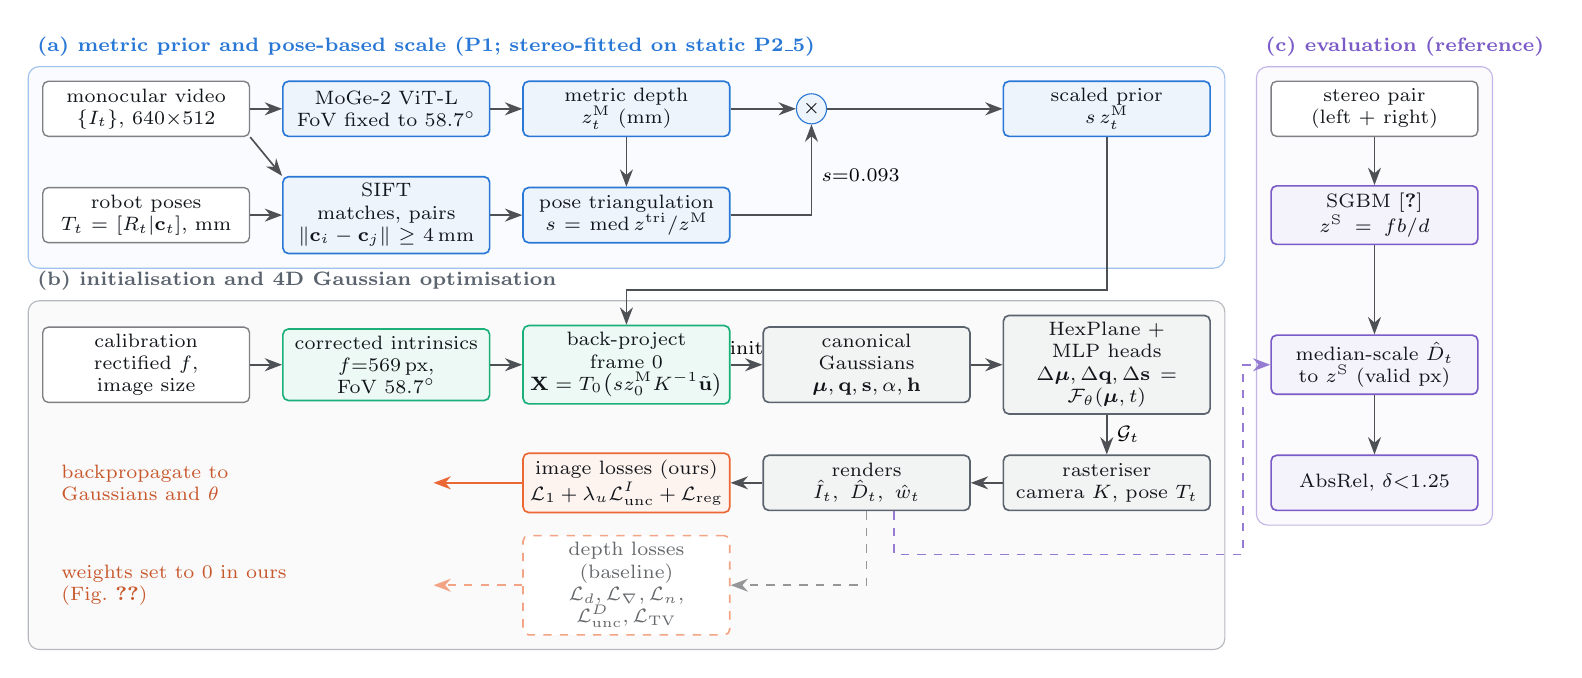
\begin{tikzpicture}[x=1cm,y=1cm, blk/.append style={text width=2.45cm}, io/.append style={text width=2.45cm}]
% columns
\def\cA{0} \def\cB{3.05} \def\cC{6.1} \def\cD{9.15} \def\cE{12.2} \def\cF{15.6}
% ---- lane (a): metric prior and stereo-free scale ----
\node[io]           (video)  at (\cA,0)    {monocular video\\$\{I_t\}$, 640$\times$512};
\node[blk=cPrior]   (moge)   at (\cB,0)    {MoGe-2 ViT-L\\FoV fixed to 58.7$^\circ$};
\node[blk=cPrior]   (zm)     at (\cC,0)    {metric depth\\$z^{\mathrm{M}}_t$ (mm)};
\node[circle, draw=cPrior, fill=cPrior!8, inner sep=1pt, font=\scriptsize] (mul) at (\cD-0.7,0) {$\times$};
\node[blk=cPrior]   (scaled) at (\cE,0)    {scaled prior\\$s\,z^{\mathrm{M}}_t$};
\node[io]           (poses)  at (\cA,-1.35) {robot poses\\$T_t=[R_t|\mathbf{c}_t]$, mm};
\node[blk=cPrior]   (sift)   at (\cB,-1.35) {SIFT matches, pairs\\$\|\mathbf{c}_i-\mathbf{c}_j\|\ge 4$\,mm};
\node[blk=cPrior]   (tri)    at (\cC,-1.35) {pose triangulation\\$s=\mathrm{med}\,z^{\mathrm{tri}}/z^{\mathrm{M}}$};
\draw[arr] (video) -- (moge);
\draw[arr] (moge) -- (zm);
\draw[arr] (zm) -- (mul);
\draw[arr] (mul) -- (scaled);
\draw[arr] (poses) -- (sift);
\draw[arr] (sift) -- (tri);
\draw[arr] (zm) -- (tri);
\draw[arr] (video.south east) -- (sift.north west);
\draw[arr] (tri.east) -| node[pos=0.72, right, font=\scriptsize]{$s{=}0.093$} (mul.south);
% ---- lane (b): initialisation and 4D Gaussian optimisation ----
\node[io]           (calib)  at (\cA,-3.25) {calibration\\rectified $f$, image size};
\node[blk=cInit]    (K)      at (\cB,-3.25) {corrected intrinsics\\$f{=}569$\,px, FoV 58.7$^\circ$};
\node[blk=cInit]    (bp)     at (\cC,-3.25) {back-project frame 0\\$\mathbf{X}=T_0\big(s z^{\mathrm{M}}_0 K^{-1}\tilde{\mathbf{u}}\big)$};
\node[blk=cModel]   (canon)  at (\cD,-3.25) {canonical Gaussians\\$\bm{\mu},\mathbf{q},\mathbf{s},\alpha,\mathbf{h}$};
\node[blk=cModel]   (def)    at (\cE,-3.25) {HexPlane + MLP heads\\$\Delta\bm{\mu},\Delta\mathbf{q},\Delta\mathbf{s}=\mathcal{F}_\theta(\bm{\mu},t)$};
\node[blk=cModel]   (rast)   at (\cE,-4.75) {rasteriser\\camera $K$, pose $T_t$};
\node[blk=cModel]   (out)    at (\cD,-4.75) {renders\\$\hat{I}_t,\ \hat{D}_t,\ \hat{w}_t$};
\node[blk=cLoss]    (img)    at (\cC,-4.75) {image losses (ours)\\$\mathcal{L}_1+\lambda_u\mathcal{L}^{I}_{\mathrm{unc}}+\mathcal{L}_{\mathrm{reg}}$};
\node[blk=cLoss, fill=white, draw=cLoss!60, dashed, text=ink!65] (dep) at (\cC,-6.05) {depth losses (baseline)\\$\mathcal{L}_d,\mathcal{L}_\nabla,\mathcal{L}_n,$\\$\mathcal{L}^{D}_{\mathrm{unc}},\mathcal{L}_{\mathrm{TV}}$};
\node[font=\scriptsize, text=cLoss!85!black, text width=2.9cm, align=left, anchor=west] (off) at (\cA-1.2,-6.05) {weights set to 0 in ours\\(Fig.~\ref{fig:loss})};
\node[font=\scriptsize, text=cLoss!85!black, text width=2.9cm, align=left, anchor=west] (bpl) at (\cA-1.2,-4.75) {backpropagate to\\Gaussians and $\theta$};
\draw[arr] (calib) -- (K);
\draw[arr] (K) -- (bp);
\draw[arr] (bp) -- node[above, font=\scriptsize]{init} (canon);
\draw[arr] (canon) -- (def);
\draw[arr] (def) -- node[right, font=\scriptsize]{$\mathcal{G}_t$} (rast);
\draw[arr] (rast) -- (out);
\draw[arr] (out) -- (img);
\draw[darr] (out.south) |- (dep.east);
\draw[arr, draw=cLoss] (img.west) -- (bpl.east -| {(\cB+0.6,0)});
\draw[arr, draw=cLoss!60, dashed] (dep.west) -- (off.east -| {(\cB+0.6,0)});
\draw[arr] (scaled.south) -- (scaled.south |- {(0,-2.3)}) -| (bp.north);
% ---- lane (c): evaluation ----
\node[io]          (stereo) at (\cF,0)     {stereo pair\\(left + right)};
\node[blk=cEval]   (sgm)    at (\cF,-1.35) {SGBM~\cite{hirschmuller2008sgm}\\$z^{\mathrm{S}}=fb/d$};
\node[blk=cEval]   (med)    at (\cF,-3.25) {median-scale $\hat{D}_t$\\to $z^{\mathrm{S}}$ (valid px)};
\node[blk=cEval]   (met)    at (\cF,-4.75) {AbsRel, $\delta{<}1.25$};
\draw[arr] (stereo) -- (sgm); \draw[arr] (sgm) -- (med); \draw[arr] (med) -- (met);
\draw[darr, draw=cEval!80] (out.south) ++(0.35,0) |- ++(0,-0.55) -| ($(med.west)+(-0.35,0)$) -- (med.west);
% ---- lanes ----
\begin{scope}[on background layer]
\node[lane=cPrior, fit=(video)(moge)(zm)(scaled)(poses)(sift)(tri), inner ysep=5pt, inner xsep=5pt] (L1) {};
\node[lane=cModel, fit=(calib)(K)(bp)(canon)(def)(rast)(out)(img)(dep)(off)(bpl), inner ysep=5pt, inner xsep=5pt] (L2) {};
\node[lane=cEval, fit=(stereo)(sgm)(med)(met), inner ysep=5pt, inner xsep=5pt] (L3) {};
\end{scope}
\node[lanelbl=cPrior, anchor=south west] at (L1.north west) {(a) metric prior and pose-based scale (P1; stereo-fitted on static P2\_5)};
\node[lanelbl=cModel, anchor=south west] at (L2.north west) {(b) initialisation and 4D Gaussian optimisation};
\node[lanelbl=cEval, anchor=south west] at (L3.north west) {(c) evaluation (reference)};
\end{tikzpicture}}
\caption{Overview. (a)~MoGe-2 predicts metric depth given the calibrated field of view; one global scale $s$ is estimated by triangulating SIFT matches with the known poses (P1). On the static P2\_5 clip, where triangulation has no parallax, $s$ is instead fitted to stereo on training frames (Section~\ref{sec:p25}). (b)~The scaled depth of the first frame, back-projected with the corrected intrinsics, initialises canonical Gaussians, which a HexPlane deformation field moves over time; training uses image losses only (solid), whereas the Endo-4DGS baseline also applies the depth-based losses (dashed). (c)~Rendered depth is compared with stereo-reference depth; on P1 stereo is used only here.}
\label{fig:pipeline}
\end{figure*}

\subsection{Problem setting and notation}
The input is a monocular video $\{I_t\}_{t=1}^{N}$ of $H{\times}W{=}512{\times}640$ rectified frames with timestamps $t/N\in[0,1)$ and camera-to-world poses $T_t=[R_t\,|\,\mathbf{c}_t]$ from the robot kinematics, in millimetres. We use the StereoMIS~\cite{hayoz2023stereomis} sequence P1, frames 801--1000 ($N{=}200$). Every eighth frame, starting with the second ($(i-1)\bmod 8=0$ for 0-based index $i$; frames 802, 810, \dots, 994), is held out for testing, leaving 175 training frames. We distinguish two input protocols. \emph{P1 (monocular):} the method uses the left images and the known metric poses only; the right stereo image is used only for evaluation. \emph{P2\_5 (stereo-assisted scale):} on the second, static clip (Section~\ref{sec:p25}) the prior scale is fitted to stereo depth on training frames, so stereo also enters initialisation.

\subsection{Camera model}
\label{sec:intrinsics}
The renderer uses a pinhole camera with horizontal field of view $\mathrm{FoV}_x=2\arctan\!\big(W/(2f)\big)$ and the principal point at the image centre. The released StereoMIS preprocessing of Endo-4DGS stores $f{=}1039.6$\,px, the focal length of the unrectified 1280$\times$1024 images, although the frames are rectified and downsampled by two. The correct value is half the rectified focal length, $f{=}1137.99/2{=}569.0$\,px. This changes $\mathrm{FoV}_x$ from 34.2$^\circ$ to 58.7$^\circ$. We use the corrected $f$ for MoGe-2, back-projection and rendering. Two intrinsic matrices remain: as in Endo-4DGS, rendering and back-projection use $K_{\mathrm{render}}$ with the principal point at the image centre $(320, 256)$, whereas the scale estimation of Section~\ref{sec:scale} uses the rectified $K_{\mathrm{tri}}$ with principal point $(327.34, 251.33)$, i.e.\ offsets of $(+7.34,-4.67)$\,px. MoGe-2 receives only the horizontal FoV. We did not test the effect of the residual offset on the renderer.

\subsection{Metric geometry prior}
\label{sec:prior}
For each frame we run MoGe-2~\cite{wang2025moge2} (ViT-L with normal head, \texttt{moge-2-vitl-normal}) at its default resolution level and provide the calibrated horizontal FoV of 58.7$^\circ$ at inference. It returns a metric depth map $z^{\mathrm{M}}_t$, a validity mask and surface normals. We convert depth to millimetres and set invalid pixels to zero; they are excluded from initialisation. Its metric scale does not transfer to these images: on the test frames the median ratio of stereo-reference depth to MoGe-2 depth is 0.168 on P1 and 0.056 on P2\_5, i.e.\ MoGe-2 depth is 6.0$\times$ and 17.8$\times$ too large (Table~\ref{tab:priors}), and the ratio varies between frames (coefficient of variation 12.8\,\% and 6.4\,\%). After per-frame median alignment its shape agrees better with the stereo reference than the Depth-Anything~\cite{yang2024depthanything} depth used by Endo-4DGS (aligned AbsRel 0.148 vs.\ 0.237 on P1).

\subsection{Stereo-free scale from pose triangulation}
\label{sec:scale}
We estimate one global factor $s$, a unit conversion that maps $z^{\mathrm{M}}$ into the metric frame of the poses (Fig.~\ref{fig:scale}). This assumes that matched points move little between the two frames compared with the camera-induced parallax; deformation, breathing, instruments and reflections violate it, so we filter correspondences geometrically. For frame pairs $(i,j)$ from a pool sampled every 5 frames, whose camera centres are at least 4\,mm apart, we match SIFT features (4000 per frame, ratio test 0.75) and reject outliers with a RANSAC fundamental matrix (1\,px threshold). We then keep only matches that are consistent with the \emph{known} poses (Sampson distance $\le$2\,px to the fundamental matrix implied by $T_i,T_j$), triangulate in front of both cameras and reproject within 2\,px in both views. Each remaining match $(\mathbf{u}_k,\mathbf{u}'_k)$ is triangulated with the projection matrices
\begin{equation}
P_i=K_{\mathrm{tri}}\,[\,R_i^{\top}\;|\;-R_i^{\top}\mathbf{c}_i\,],\qquad P_j=K_{\mathrm{tri}}\,[\,R_j^{\top}\;|\;-R_j^{\top}\mathbf{c}_j\,],
\end{equation}
which gives a depth $z^{\mathrm{tri}}_k$ in camera $i$. The scale is the median of per-pair medians,
\begin{equation}
s=\operatorname*{median}_{(i,j)}\;\operatorname*{median}_{k}\;\frac{z^{\mathrm{tri}}_k}{z^{\mathrm{M}}_i(\mathbf{u}_k)} ,
\label{eq:scale}
\end{equation}
where we keep only pairs with at least 20 valid ratios. The triangulated depth is computed independently of the prior, but $s$ divides by the prior and therefore inherits its frame-to-frame scale variation.

\emph{Frame pool and sensitivity.} The experiments of Sections~\ref{sec:results}--\ref{sec:explain} use $s{=}0.0928$, which was estimated before we restricted the pool and added the known-pose filters: it used all 200 frames, including the 25 test frames, and only the RANSAC filter (144 pairs, inter-quartile range 0.085--0.107). With training frames only it becomes 0.0976 (116 pairs), and with the known-pose filters 0.1044 (51 pairs, 35 training frames 801, 806, \dots; IQR 0.087--0.108). The cheirality, reprojection and triangulation-angle ($\geq$1--2$^\circ$) filters remove no further pairs. The estimate is stable for baselines of at least 4\,mm (0.1044 at 4\,mm, 0.1054 at 6\,mm with IQR 0.105--0.108) but biased low at 2\,mm (0.085, IQR 0.065--0.104). We retrain our model with the held-out-clean factor 0.1044 in Section~\ref{sec:results} to check that the conclusions do not depend on the test frames. The factor differs from the stereo fit on P1 (0.165); candidate explanations are kinematic pose error (2--6\,px epipolar error between robot poses and image matches), tissue motion and the different pixel sets used by the two fits, and we do not attribute the gap to one of them. A single factor converts units consistently with the poses; it does not correct the frame-to-frame scale variation of MoGe-2, and our model initialises from one frame only. Solving for $s$ directly from back-projected prior points, $s\,(R_iP^{\mathrm{M}}_i-R_jP^{\mathrm{M}}_j)=\mathbf{c}_j-\mathbf{c}_i$, failed in our setting (estimates of 0.006--0.026) because the $\sim$10\,mm error of the prior overwhelms baselines of a few millimetres.

\begin{figure}[t]
\centering
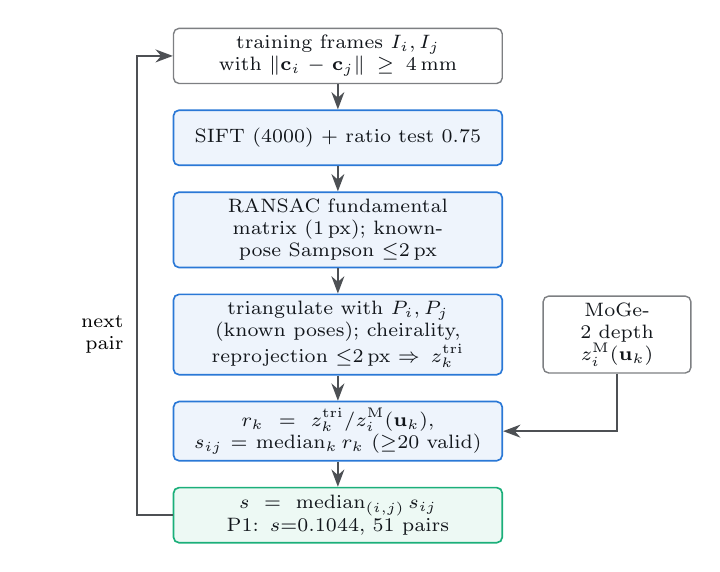
\begin{tikzpicture}[node distance=3.2mm, every node/.append style={text width=4.0cm}]
\node[io] (pair) {training frames $I_i, I_j$ with $\|\mathbf{c}_i-\mathbf{c}_j\|\geq 4$\,mm};
\node[blk=cPrior, below=of pair] (sift) {SIFT (4000) + ratio test 0.75};
\node[blk=cPrior, below=of sift] (ransac) {RANSAC fundamental matrix (1\,px); known-pose Sampson $\le$2\,px};
\node[blk=cPrior, below=of ransac] (tri) {triangulate with $P_i, P_j$ (known poses); cheirality, reprojection $\le$2\,px $\Rightarrow z^{\mathrm{tri}}_k$};
\node[io, right=5mm of tri, text width=1.7cm] (prior) {MoGe-2 depth $z^{\mathrm{M}}_i(\mathbf{u}_k)$};
\node[blk=cPrior, below=of tri] (ratio) {$r_k=z^{\mathrm{tri}}_k/z^{\mathrm{M}}_i(\mathbf{u}_k)$, \ $s_{ij}=\mathrm{median}_k\, r_k$ ($\geq$20 valid)};
\node[blk=cInit, below=of ratio] (s) {$s=\mathrm{median}_{(i,j)}\, s_{ij}$ \quad P1: $s{=}0.1044$, 51 pairs};
\draw[arr] (pair) -- (sift); \draw[arr] (sift) -- (ransac); \draw[arr] (ransac) -- (tri);
\draw[arr] (tri) -- (ratio); \draw[arr] (prior) |- (ratio.east); \draw[arr] (ratio) -- (s);
\coordinate (lx) at ($(tri.west)+(-0.45,0)$);
\draw[arr] (s.west) -- (s.west -| lx) -- (pair.west -| lx) -- (pair.west);
\node[font=\scriptsize, text width=1.1cm, align=right, anchor=east] at ($(lx)+(-0.05,0)$) {next\\pair};
\end{tikzpicture}
\caption{Estimation of the global prior scale $s$ from known poses and inter-frame matches (Eq.~\ref{eq:scale}); stereo depth is not used. Shown with the corrected frame pool and filters; the main experiments used $s{=}0.0928$ from the earlier, unfiltered all-frame estimate (Section~\ref{sec:scale}).}
\label{fig:scale}
\end{figure}

\subsection{Initialisation}
The canonical Gaussians are created by back-projecting the scaled prior of the first training frame with the corrected intrinsics,
\begin{equation}
\mathbf{X}(\mathbf{u})=R_0\,\big(s\,z^{\mathrm{M}}_0(\mathbf{u})\,K^{-1}\tilde{\mathbf{u}}\big)+\mathbf{c}_0 ,
\end{equation}
for every pixel $\mathbf{u}$ with valid prior depth that is not masked as an instrument, using $K_{\mathrm{render}}$. Here $\tilde{\mathbf{u}}$ is the homogeneous pixel coordinate, and each point takes the pixel's colour as its initial colour. This yields at most 327\,680 Gaussians for a 640$\times$512 frame; on P1 all pixels of the first training frame (801) are valid and unmasked, so the initial count is exactly 327\,680 (the final count after densification and pruning is reported separately in Table~\ref{tab:hw}). The baseline is initialised the same way from its Depth-Anything depth (the inverse of the predicted disparity, scaled by $10^3$ and clipped to its 5th--95th percentiles) and the uncorrected intrinsics.

\subsection{Deformable 4D Gaussian representation}
Each Gaussian $k$ has a mean $\bm{\mu}_k$, rotation quaternion $\mathbf{q}_k$, scale $\mathbf{s}_k$, opacity $\alpha_k$ and spherical-harmonic colour $\mathbf{h}_k$ (degree~3), with covariance $\Sigma_k=R(\mathbf{q}_k)S(\mathbf{s}_k)S(\mathbf{s}_k)^{\top}R(\mathbf{q}_k)^{\top}$. Following Endo-4DGS and 4DGS~\cite{huang2024endo4dgs,wu2024_4dgs}, a deformation field maps a canonical Gaussian to time $t$:
\begin{equation}
(\Delta\bm{\mu}_k,\Delta\mathbf{q}_k,\Delta\mathbf{s}_k)=\mathcal{F}_\theta\big(\mathrm{HexPlane}(\bm{\mu}_k,t)\big),
\end{equation}
where HexPlane features come from six 2D planes over $(x,y,z,t)$ at resolution 64$\times$64$\times$64$\times$75 with 32 channels and two multi-resolution levels, and $\mathcal{F}_\theta$ consists of small MLP heads of width 64. Opacity and colour are not deformed. With the compositing weights $a_k(\mathbf{p})=\alpha'_k\prod_{l<k}(1-\alpha'_l)$ of the depth-sorted Gaussians, the rasteriser returns
\begin{equation}
\begin{aligned}
\hat{I}(\mathbf{p})&=\textstyle\sum_k a_k\mathbf{c}_k+\big(1-\sum_k a_k\big)\mathbf{b},\\
\hat{w}(\mathbf{p})&=\textstyle\sum_k a_k,\qquad
\hat{D}(\mathbf{p})=\sum_k a_k z_k\,\big/\,\hat{w}(\mathbf{p}),
\end{aligned}
\end{equation}
with background colour $\mathbf{b}$ and camera-space depths $z_k$. $\hat{D}$ is the opacity-normalised expected depth along the ray, not necessarily the first surface intersection; pixels with $\hat{w}{=}0$ have no depth and are excluded from all depth metrics. Endo-4DGS uses the accumulated opacity $\hat{w}$ as a confidence map.

\subsection{Training objective}
\label{sec:objective}
Endo-4DGS minimises
\begin{equation}
\begin{aligned}
\mathcal{L}=\;&\mathcal{L}_1(\hat{I},I)+\lambda_u\mathcal{L}^{I}_{\mathrm{unc}}+\mathcal{L}_{\mathrm{reg}}\\
&+\underbrace{\lambda_d\big(\mathcal{L}_{d}+\mathcal{L}_{\nabla}+\mathcal{L}_{\mathrm{TV}}\big)+\lambda_n\mathcal{L}_{n}+\lambda_u\mathcal{L}^{D}_{\mathrm{unc}}}_{\text{depth-based terms}} .
\end{aligned}
\label{eq:loss}
\end{equation}
Here $\mathcal{L}_d$ is an L1 loss between max-normalised rendered and prior depth, $\mathcal{L}_\nabla$ a depth-gradient loss, $\mathcal{L}_{\mathrm{TV}}$ total variation of the rendered depth and image, and $\mathcal{L}_n$ an L1 loss between rendered normals and pseudo-normals from prior-depth gradients. The uncertainty terms are computed with global reductions over the valid pixels $\mathcal{V}$,
$\mathcal{L}^{I}_{\mathrm{unc}}=\big(\tfrac{1}{|\mathcal{V}|}\sum_{\mathbf{p}}\|\hat{I}-I\|^2\big)\big/\big(\tfrac{2}{|\mathcal{V}|}\sum_{\mathbf{p}}\hat{w}^2\big)+\tfrac{1}{|\mathcal{V}|}\sum_{\mathbf{p}}\log\hat{w}$,
and likewise $\mathcal{L}^{D}_{\mathrm{unc}}$ on max-normalised depth; a pixel's error is therefore not weighted by its own $\hat{w}$, and $\hat{w}$ is not trained as a calibrated per-pixel error estimate. Finally, $\mathcal{L}_{\mathrm{reg}}$ regularises the HexPlanes with spatial total variation, temporal smoothness and L1 on the time planes. Fig.~\ref{fig:loss} lists the weights. The max-normalised terms $\mathcal{L}_d$ and $\mathcal{L}^{D}_{\mathrm{unc}}$ are invariant to a multiplicative depth scale; the pseudo-normals (built from raw prior-depth differences, $[\partial_x z, -\partial_y z, -1]$ normalised) and the total variation of the rendered depth are evaluated in raw depth units and are not, and the image TV term shares the weight $\lambda_d$ in the released code. With the scaled MoGe-2 initialisation we set $\lambda_d$, $\lambda_n$ and the depth-uncertainty weight to zero, which disables the depth, depth-gradient, depth-TV and image-TV, pseudo-normal and depth-uncertainty terms \emph{together}; Section~\ref{sec:results} shows that removing this group improves PSNR, but does not isolate the effect of each term.

\begin{figure}[t]
\centering
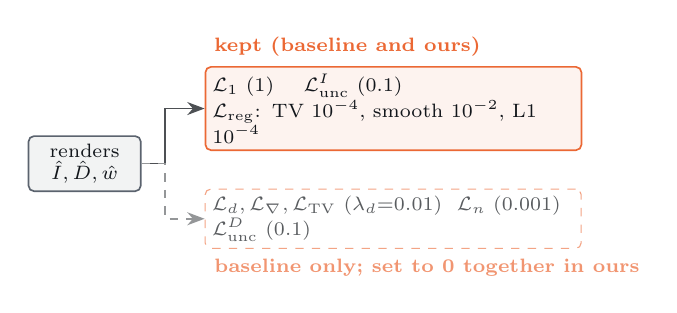
\begin{tikzpicture}[node distance=2.4mm]
\node[blk=cModel, text width=1.25cm] (r) {renders\\$\hat{I},\hat{D},\hat{w}$};
\node[blk=cLoss, right=8mm of r, yshift=7mm, text width=4.6cm, align=left] (on) {$\mathcal{L}_1$ (1) \quad $\mathcal{L}^{I}_{\mathrm{unc}}$ (0.1)\\$\mathcal{L}_{\mathrm{reg}}$: TV $10^{-4}$, smooth $10^{-2}$, L1 $10^{-4}$};
\node[draw=cLoss!60, dashed, rounded corners=2pt, fill=white, font=\scriptsize, align=left, inner sep=2.5pt, text width=4.6cm, right=8mm of r, yshift=-7mm, text=ink!70] (off) {$\mathcal{L}_d,\mathcal{L}_\nabla,\mathcal{L}_{\mathrm{TV}}$ ($\lambda_d{=}0.01$) \ $\mathcal{L}_n$ (0.001)\\$\mathcal{L}^{D}_{\mathrm{unc}}$ (0.1)};
\draw[arr] (r.east) -- ++(3mm,0) |- (on.west);
\draw[darr] (r.east) -- ++(3mm,0) |- (off.west);
\node[font=\scriptsize\bfseries, text=cLoss, anchor=south west] at (on.north west) {kept (baseline and ours)};
\node[font=\scriptsize\bfseries, text=cLoss!70, anchor=north west] at (off.south west) {baseline only; set to 0 together in ours};
\end{tikzpicture}
\caption{Loss terms and weights (Eq.~\ref{eq:loss}). Our model keeps only the image and HexPlane terms; note that $\lambda_d$ also scales the image TV term.}
\label{fig:loss}
\end{figure}

\subsection{Optimisation}
Training follows Endo-4DGS: 2000 coarse iterations without deformation, then 6000 fine iterations with deformation, batch size 1. Gaussians are densified and pruned every 100 iterations between iterations 500 and 3000, and opacity is never reset. Learning rates are the Endo-4DGS defaults; for example, the position rate decays from $1.6{\times}10^{-4}$ to $1.6{\times}10^{-6}$, the deformation MLP rate from $1.6{\times}10^{-4}$ to $1.6{\times}10^{-6}$ and the HexPlane rate from $1.6{\times}10^{-3}$ to $1.6{\times}10^{-5}$. One run takes about 16\,min on a single RTX 4060 Ti, and the trained model renders at 38\,FPS.

\subsection{Geometric evaluation protocol}
\label{sec:evalproto}
Image quality is reported as PSNR, SSIM and LPIPS (AlexNet) on the 25 test frames. No ground-truth surface is available, so we compare against a \emph{stereo reference}: depth estimated from the rectified stereo pair with semi-global block matching~\cite{hirschmuller2008sgm}, using 256 disparities, block size 5, smoothness penalties $P_1{=}600$ and $P_2{=}2400$, uniqueness ratio 10 and speckle filtering (window 100, range 2), and $z^{\mathrm{S}}=fb/d$ with $fb{=}2494.6$\,px$\cdot$mm at 640$\times$512. Our main geometric metric is a \emph{shape} diagnostic: each rendered depth map $\hat{D}_t$ is multiplied by $\mathrm{median}(z^{\mathrm{S}}/\hat{D}_t)$ over $\Omega$ before computing
\begin{align}
\mathrm{AbsRel}&=\frac{1}{|\Omega|}\sum_{\mathbf{p}\in\Omega}\frac{|\hat{D}(\mathbf{p})-z^{\mathrm{S}}(\mathbf{p})|}{z^{\mathrm{S}}(\mathbf{p})},\\
\delta&=\frac{1}{|\Omega|}\sum_{\mathbf{p}\in\Omega}\Big[\max\!\Big(\frac{\hat{D}(\mathbf{p})}{z^{\mathrm{S}}(\mathbf{p})},\frac{z^{\mathrm{S}}(\mathbf{p})}{\hat{D}(\mathbf{p})}\Big)<1.25\Big],
\end{align}
where $\Omega$ is the set of pixels with SGBM disparity $>1$\,px (valid stereo depth; $\approx$50\,\% of each frame, the leftmost 256 columns being outside the disparity search range) and finite, positive rendered depth. We call this the \emph{per-frame scale-aligned, stereo-reference-relative} AbsRel. Per-frame alignment removes absolute and frame-to-frame scale errors, which matter because the poses are metric. We therefore also report the \emph{metric} AbsRel of the raw rendered depth, the AbsRel after \emph{one} scale factor fitted on the training views, and the statistics of the per-frame factors (Table~\ref{tab:metric}). Metrics are averaged over the test frames and then over three training seeds; $\pm$ denotes the sample standard deviation over seeds ($n{-}1$).

\subsection{Variants examined}
\textbf{MoGe-2 normal supervision.} We replace $\mathcal{L}_n$ by a cosine loss between rendered and MoGe-2 normals. Each Gaussian's normal (the axis of its smallest scale) is rotated into the camera frame, flipped to face the camera and composited on a black background. This removes the view-dependent colour terms and the white-background bias that affect the baseline's normal map. The loss is $\lambda\,(1-\langle\hat{\mathbf{n}},\mathbf{n}^{\mathrm{M}}\rangle)$, averaged over valid pixels, with $\lambda\in\{0.01,0.05\}$.

\textbf{Bundle-adjusted poses.} Starting from the robot poses, we triangulate exhaustive SIFT matches and run COLMAP~\cite{schonberger2016sfm} bundle adjustment with fixed intrinsics. We align the result back to the robot frame: the rotation is the chordal mean of the per-camera offsets, and the scale and offset come from a least-squares fit of the camera centres. Optionally, only a temporally smoothed correction is applied (a Gaussian filter with $\sigma{=}15$ frames on the per-frame rotation vector and translation offset).

\bibliographystyle{IEEEtran}
\bibliography{refs}
\end{document}
